\section{Mekanikk}
\comment{\subsection{Reaksjoner i systemet}}

For å utvikle ideer til hvordan problemstillingen kan løses, er det nødvendig å analysere hva som skjer om en hjulmutter løsner. Det har i denne sammenheng blitt brukt en brainstorming-teknikk for å sammen kunne komme fram til så mange av disse reaksjonene som mulig. Vi har identifisert følgende reaksjoner grunnet endring i mutterens tilstramming:

\begin{table}[h]
\caption{Mekaniske og andre reaksjoner i systemet}
\begin{tabular}{|l|l|}
\hline
\textbf{Mekanisk}                   & \textbf{Annet}                                   \\
\hline
Strekk i bolt ved strammet mutter   & Temperaturendring pga friksjonsvarme ved løsning \\
\hline
Kompresjonsendring i mutter         & Vibrasjonsendringer i understell                 \\
\hline
Torsjonsendring                     & Endring i friksjon mellom bakke og hjul          \\
\hline
Trykkendring mellom mutter og flate & ...                                              \\
\hline
\end{tabular}
\end{table}

\subsection{Håndberegninger av strekk og trykk}

Etter å ha intervjuet Olav Rogne, yrekssjåfør, har vi valgt å bruke dimensjonene han har oppgitt som utregningseksempel. Det ble opplyst om at det var normalt å bruke mutter av typen M33x3.5 som trekkes til med et tiltrekkingsmoment på 700Nm. Man kan utifra dette enkelt regne ut spenninger som oppstår i bolten.

Momentet som tilføres bolten ved tiltrekking deles opp i to komponenter:
\begin{center}
$M_{tiltrekning}=M_{v}+M_{s}$
\end{center}
Der $M_{v}$ er momentet som oppstår pga friksjonskrefter i gjengeflaten, og $M_{s}$ er momentet som oppstår pga krefter mellom mutter og underlaget. Disse kan igjen bli beskrevet slik:
\begin{center}
$M_{v}=F\cdot tan(\varphi +\varepsilon )\cdot r_{m}$
\end{center}
og
\begin{center}
$M_{s}=\mu 'Fr_{m}$
\end{center}
I disse to formlene tar vi i bruk flere fraktorer. $ r_{m}$ er radiusen som friksjonskraften mot underlaget antas å virke på:
\begin{center}
$r_{m}=\frac{N\o kkelvidde+d_{h}}{4}$
\end{center}
$\varphi$ er gjengenes stigningsvinkel:
\begin{center}
$\varphi =\frac{gjengestigning}{\pi \cdot d_{pich}}$
\end{center}
og $\varepsilon$ er friksjonsvinkelen i skråplanet der kreftene i gjengene virker:
\begin{center}
$\varepsilon =tan^{-1}(\frac{\mu}{cos(\alpha )})$
\end{center}
Her er $\alpha$ halve gjengevinkelen og vi har satt friksjonsfaktor i gjengeene til $\mu=0.08$ \cite{FriksjonsfaktorGjenger} %http://www.kamax.com/fileadmin/user_upload/dokumente/pdf/Bolt_and_Screw_Compendium.pdf

Videre kan vi løse dette for kraften:
\begin{center}
$F_{aksiell}=\frac{M_{tiltrekning}}{(tan(\varphi +tan^{-1}(\frac{\mu }{cos(\alpha )}))+\mu')\frac{N+d_{h}}{4}}$
\end{center}
Siden vi også vet at
\begin{center}
$\sigma=\frac{F}{A}$
\end{center}
Kan vi si at trykket mellom mutter og underlag er:
\begin{center}
$p_{trykkflate}=\frac{F_{aksiell}}{A_{trykkflate}}=\frac{F_{aksiell}}{\frac{\pi }{4}(D_{mutterflate}^{2}-D_{hull}^{2})}$
\end{center}
Videre vet vi at flytegrensen er:

\begin{center}
$\sigma _{f}\approx 250 Mpa-350 Mpa$
\end{center}

Ut ifra disse beregningene har vi kommet fram til at det vil være et overtrykk trykk på 116.6 MPa mellom mutter og flaten mutteren trykker på, samt et strekk på 193 Mpa i bolten.

\subsection{FEM-analyse}

Beregningene i forrige avsnitt kan også simuleres med en "finite element method" (FEM) analyse i programvare tilgjengelig ved NTNU som for eksempel NX 9.0 som er brukt i dette tilfellet. Først blir bolten og mutteren modellert etter dimensjonene for en M33x3.5 bolt. Den blir så tilført et mesh av elementer. Disse elementene blir hver for seg oppfattet som en egen modell, der beregninger blir gjennomført på et og et element, der reaksjonene i elementenes noder blir overført til sammenfallende noder i omliggende elementer. På denne måten kan man simulere hvordan krefter virker på både bolt og mutter slik at man får ut ønskede reaksjoner.

\begin{figure}[H]
		\centering
		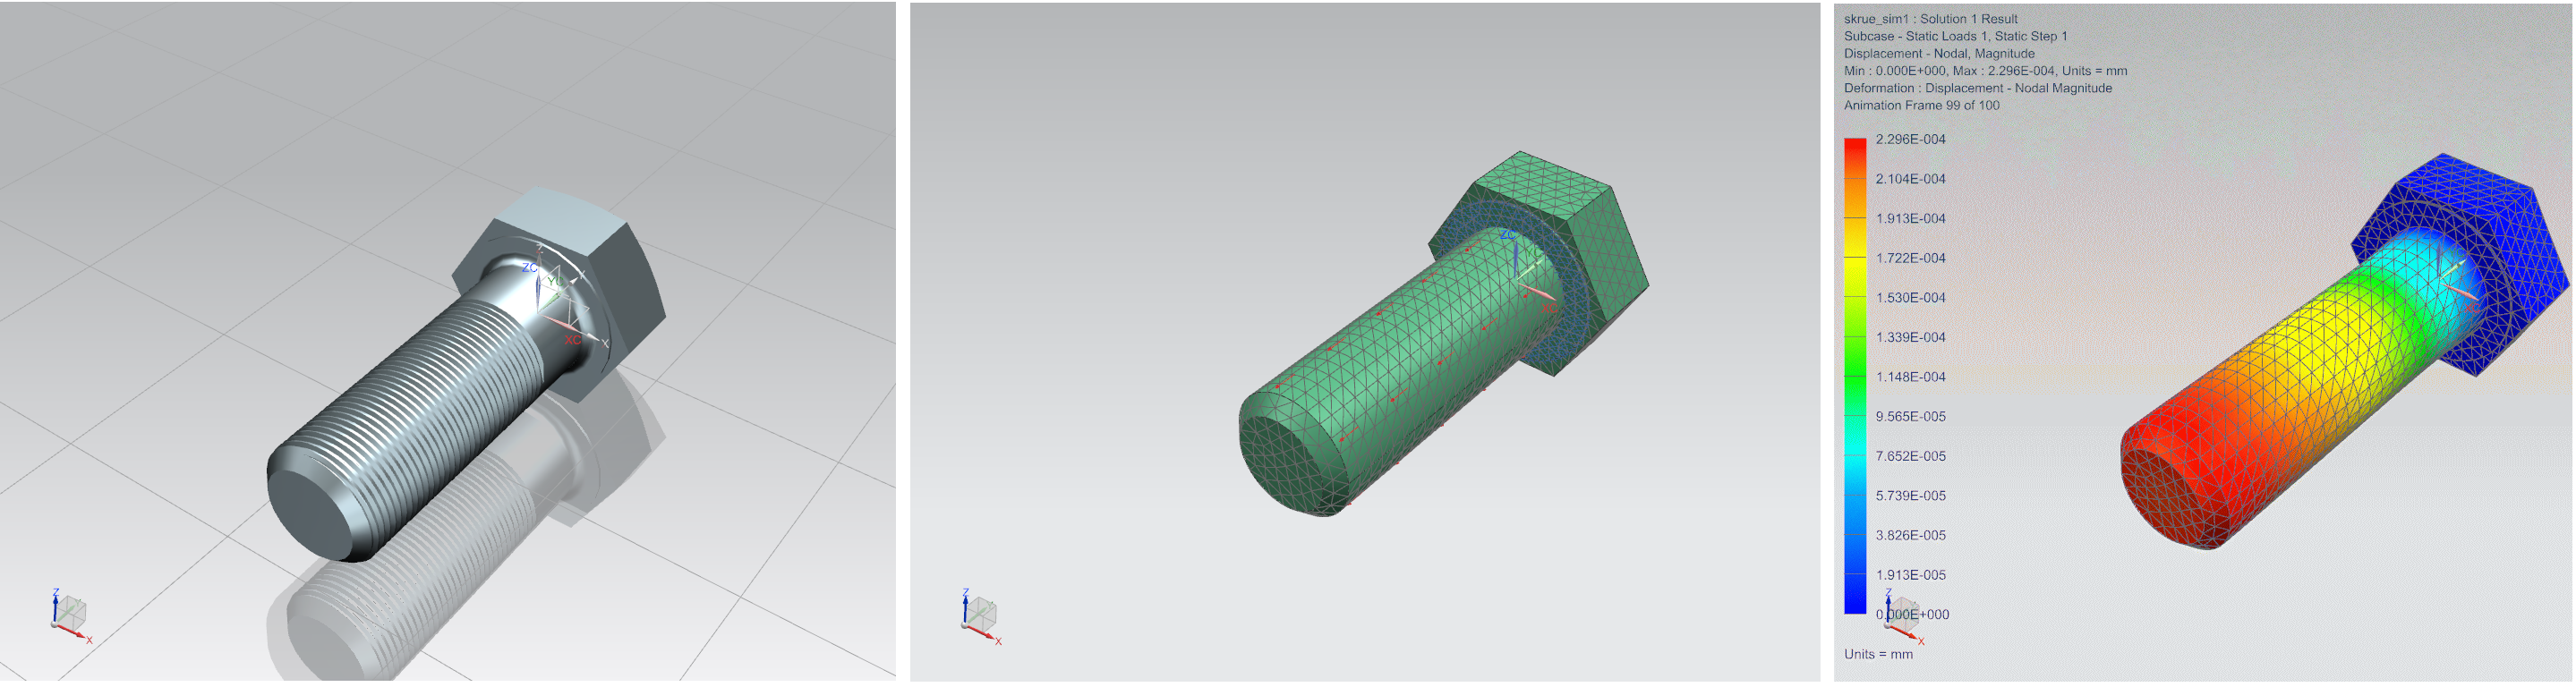
\includegraphics[width=1.00\textwidth]{images/Rapportbilde_skrue.png}
		\label{fig:FEMskrue}
		\caption{FEM-analyse av belastninger på tiltrukket bolt. Fra venstre til høyre: Modellert bolt, Forenklet og tilført mesh, Styrkeberegninger (her illustrert ved deformasjon}
	\end{figure}
\begin{figure}[H]
		\centering
		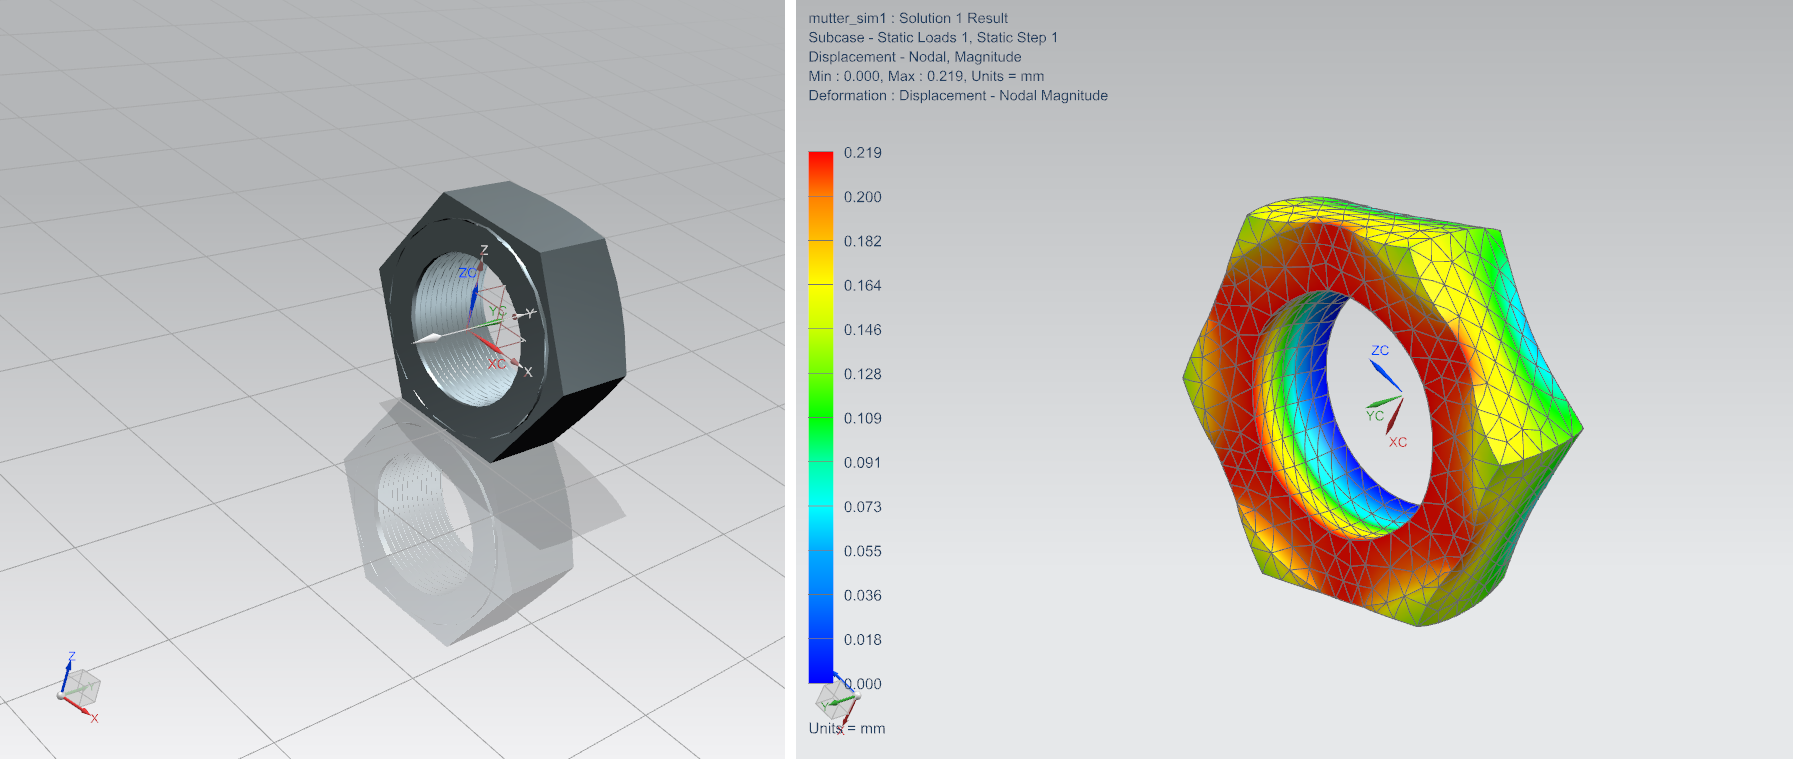
\includegraphics[width=1.00\textwidth]{images/Rapportbilde_mutter.png}
		\label{fig:FEMmutter}
		\caption{FEM-analyse av belastninger på tiltrukket mutter. Fra venstre til høyre: Modellert mutter, Styrkeberegninger her illustrert ved deformasjon.}
	\end{figure}

 